\documentclass[12pt,italian]{report}
\usepackage{tesi}
%\usepackage[section]{placeins}

%
%			INFORMAZIONI SULLA TESI
%			DA COMPILARE!
%

% CORSO DI LAUREA:
\def\myCDL{Corso di Laurea magistrale in\\Informatica}
% TITOLO TESI:
\def\myTitle{Il titolo\\della tesi}

% AUTORE:
\def\myName{Lorenzo D'Alessandro}
\def\myMat{Matr. Nr. 939416}

% RELATORE E CORRELATORE:
\def\myRefereeA{Relatore 1}
\def\myRefereeB{Correlatore 1}

% ANNO ACCADEMICO
\def\myYY{2020-2021}

% Il seguente comando introduce un elenco delle figure dopo l'indice (facoltativo)
%\figurespagetrue

% Il seguente comando introduce un elenco delle tabelle dopo l'indice (facoltativo)
%\tablespagetrue

%
%			PREAMBOLO
%			Inserire qui eventuali package da includere o definizioni di comandi personalizzati
%

% Package di formato
\usepackage[a4paper]{geometry}		% Formato del foglio
\usepackage[italian]{babel}			% Supporto per l'italiano
\usepackage[utf8]{inputenc}			% Supporto per UTF-8
%\usepackage[a-1b]{pdfx}			% File conforme allo standard PDF-A (obbligatorio per la consegna)

% Package per la grafica
\usepackage{graphicx}				% Funzioni avanzate per le immagini
\usepackage{hologo}					% Bibtex logo with \hologo{BibTeX}
%\usepackage{epsfig}				% Permette immagini in EPS
%\usepackage{xcolor}				% Gestione avanzata dei colori

% Package tipografici
\usepackage{amssymb,amsmath,amsthm} % Simboli matematici
\usepackage{listings}				% Scrittura di codice

% Package ipertesto
\usepackage{url}					% Visualizza e rendere interattii gli URL
\usepackage{hyperref}				% Rende interattivi i collegamenti interni


\begin{document}

% Creazione automatica del frontespizio
\frontespizio
\beforepreface

% 
%			PAGINA DI DEDICA E/O CITAZIONE
%			facoltativa, questa è l'unica cosa che dovete formattare a mano, un po' come vi pare
%

{\raggedleft \large \sl Dedica \\}
         
% 
%			PREFAZIONE (facoltativa)
%

%\prefacesection{Prefazione}
%Le prefazioni non sono molto comuni, tuttavia a volte capita che qualcuno voglia dire qualcosa che esuli dal lavoro in s\'e (come un meta-commento sull'elaborato), o voglia fornire informazioni riguardanti l'eventuale progetto entro cui la tesi si colloca (in questo caso \`e probabile che sia il relatore a scrivere questa parte).

%
%			RINGRAZIAMENTI (facoltativi)
%

\prefacesection{Ringraziamenti}
Questa sezione, facoltativa, contiene i ringraziamenti.

%
%			Creazione automatica dell'indice
%

\afterpreface

% 
%			CAPITOLO 1: Introduzione o Abstract
% 

\chapter{Introduzione}
\label{cap:introduzione}

Introduzione...

\section{I contenuti}
\label{sec:contenuti}

Spiegazione problema...


\section{Organizzazione della tesi}
\label{sec:organizzazione}

Organizzazione tesi...

% 
%			CAPITOLO 2: Stato dell'arte
% 



\chapter{Stato dell'arte}
\label{chap:stato_arte}
I recommender system sono algoritmi mirati a suggerire oggetti rilevanti agli utenti. La definizione di oggetto è generica e include ad esempio film da guardare, libri da leggere, prodotti da comprare o qualsiasi altra cosa a seconda del settore in cui sono implementati. 
I recommender system si dividono principalmente in 3 categorie:
\begin{itemize}
	\item collaborative filtering
	\item content based
	\item hybrid
\end{itemize}

\section{Collaborative filtering}
Collaborative filtering (CF) è considerata la tecnica di raccomandazione più popolare e ampiamente utilizzata nei RS. Il presupposto alla base di CF è che le persone con preferenze simili valuteranno gli stessi oggetti con valutazioni simili. CF quindi sfrutta le informazioni sul comportamento passato o le opinioni di una comunità di utenti esistente per prevedere quali elementi potranno piacere o saranno interessanti per l'utente corrente del sistema \cite{recsys-intro}. Gli approcci CF puri non sfruttano né richiedono alcuna conoscenza degli oggetti stessi ma solo dei feedback degli utenti. I feedback possono essere espliciti o impliciti. I feedback espliciti sono valori numerici che un utente assegna ad un prodotto, i feedback impliciti riflettono indirettamente le opinioni di un utente osservando la cronologia degli acquisti, la cronologia del browser o altro. 
La classe di algoritmi più famosa è quella di Matrix Factorization, ma recentemente sono stati sviluppati diversi approcci basati sul deep learning \cite{deep-learning-survey}.


\subsection{Matrix factorization}
Gli algoritmi basati su matrix factorization(MF) caratterizzano sia utenti che oggetti mediante dei vettori di fattori estratti dai pattern sui ratings. Una corrispondenza alta tra i fattori di un utente e un oggetto porta ad una raccomandazione. Questi metodi sono diventati popolari negli ultimi anni perchè combinano scalabilità e accuratezza.

Più formalmente, i modelli basati su matrix factorization mappano utenti e oggetti in uno spazio di fattori latenti di dimensionalità $f$, tale che le interazioni tra utenti e oggetti sono modellate come prodotti in quello spazio. Di conseguenza, ogni oggetto $i$ è associato con un vettore $q_i \in \mathbb{R}^f$, e ogni utente $u$ con un vettore $p_u \in \mathbb{R}^f$. Per un dato oggetto $i$, gli elementi di $q_i$ indicano la misura in cui l'oggetto possiede quei fattori, positivi o negativi. Per un dato utente $u$, gli elementi di $p_u$ indicato la misura di interesse che l'utente ha per gli oggetti sui fattori corrispondenti, positivi o negativi. Il prodotto scalare $q_i^Tp_u$ indica l'interesse dell'utente $u$ per le caratteristiche dell'oggetto $i$ \cite{matrix-factorization}. Quindi il rating $r_{ui}$ può essere approssimato come

\begin{equation} \label{eq:dot_product}
r_{ui} = q_i^Tp_u
\end{equation}

Il problema principale è calcolare il mapping di ogni oggetto e utente su dei vettori $q_i, p_u \in \mathbb{R}^f$. Una volta che il recommender system ha completato il mapping, può facilmente stimare il rating che un utente darà a qualsiasi oggetto utilizzando l'equazione \ref{eq:dot_product}. 

In \autoref{fig:matrix_factorization} è mostrato come la matrice dei ratings $A \in \mathbb{R}^{m \times n}$, in cui $m$ è il numero di utenti e $n$ il numero di oggetti, viene decomposta in due matrici più piccole:

\begin{itemize}
	\item Una matrice di embedding per gli utenti $P \in \mathbb{R}^{m \times f}$, in cui la riga $i$ è l'embedding dell'utente $i$
	\item Una matrice di embedding per gli oggetti $Q \in \mathbb{R}^{m \times f}$, in cui la colonna $j$ è l'embedding dell'utente $j$
\end{itemize}

\begin{figure}
  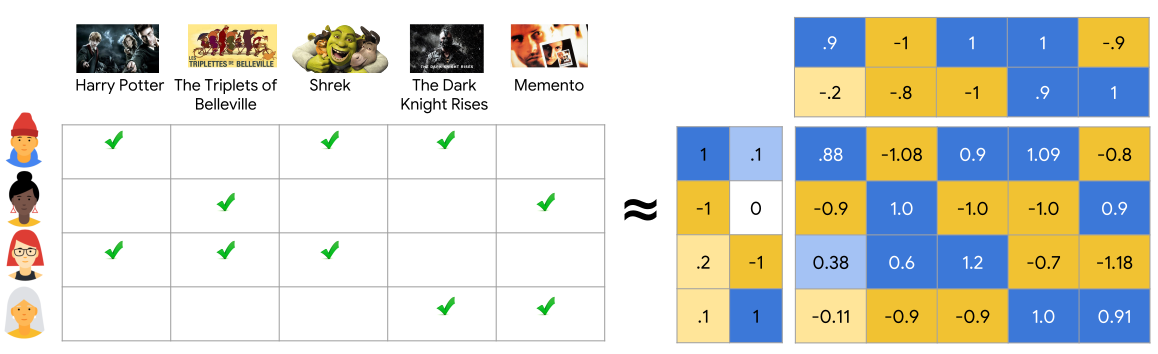
\includegraphics[width=\linewidth]{immagini/matrix_factorization.pdf}
  \caption{Approssimazione matrice dei ratings con matrix factorization}
  \label{fig:matrix_factorization}
\end{figure}

\section{Content based}
Nei recommender system content-based, gli attributi descrittivi degli oggetti sono usati per produrre raccomandazioni. Il termine "content" indica queste descrizioni. Nei metodi content-based, i ratings degli utenti sono combinati con le informazioni disponibili per gli oggetti, per poi essere usati come training data per creare un modello di classificazione o regressione specifico per l'utente. Questo modello specifico dell'utente viene utilizzato per prevedere se alla persona corrispondente piacerà un articolo per il quale la sua valutazione è ancora sconosciuta \cite{recsys-book}.





% 
%			CAPITOLO 3: Lavoro svolto
% 

\chapter{Classificatore}
\label{chap:classificatore}

\section{Introduzione}
In questo capitolo vengono descritti i problemi dell'implementazione di modelli di raccomandazione collaborative filtering in ambiente mobile. Viene poi descritto un nuovo modello che supera le limitazioni delle soluzioni proposte in letteratura, facendo comunque uso delle informazioni su users e items.

\section{Limitazioni recsys collaborative filtering}
La principale limitazione dei recommender system dei collaborative filtering è definire il numero di users e items prima di iniziare l'aggiornamento/training del modello. Nel caso degli algoritmi di matrix factorization la matrice di input è composta da un numero di righe pari al numero di users, e un numero di colonne pari al numero di items. Nel caso dei modelli basati su reti neurali descritti nel \autoref{chap:stato_arte} è necessario dare in input ai modelli le lunghezze dei vettori di users e items che corrispondono rispettivamente al numero di users e items.

In entrambi se si vuole aggiungere un nuovo user/item è necessario ricompilare il modello ed eseguire nuovamente da zero la fase di training. Questo non è un problema in un ambiente desktop in cui è possibile aggiornare giornalmente lato server le preferenze di tutti gli utenti con una cadenza regolare (es. una volta al giorno).

Eseguire di nuovo il traning da zero ogni volta che nuovi users/items vengono scoperti è un problema se si vuole fare il traning direttamente su dispositivo mobile. In questo caso c'è un problema sia di dispendio energetico, sia di tempo effettivo per il traing.

\section{Struttura classificatore}
Il modello proposto in questa tesi è una rete feed-forward fully-connected. Una rete feed-forward non contiene cicli nel suo grafo \cite{Goodfellow-et-al-2016}, mentre fully connected indica che ogni neurone in un layer è connesso a tutti i neuroni del layer successivo. Il numero di layer nascosti e il numero di neuroni in ogni layer è stato deciso nella fase di tuning descritta nel \autoref{chap:risultati}.
Il numero di neuroni nel layer di output è sempre 1 come è prassi nei problemi di classificazione binaria. La funzione di attivazione scelta per i layer nascosti è ReLU (rectified linear unit), che è più plausibile biologicamente rispetto ad altre funzioni come sigmoide o hyperbolic tangent, non viene saturata e aiuta a prevenire l'overfitting del modello \cite{rectifier-neural-networks}. La funzione di attivazione scelta per il layer di output è la sigmoide che limita l'output a valori compresi tra 0 e 1. La funzione di loss della rete è binary cross entropy. \\

L'input di un recommender system context aware solitamente è composto da:
\begin{itemize}
	\item ID user
	\item ID item
	\item informazioni di contesto
\end{itemize}

L'idea alla base del modello proposto in questa tesi è sostituire gli ID di users e items con delle features che li rappresentano. In questo modo non è necessario definire a priori il numero di users e items, e il modello può essere aggiornato senza dover ricominciare ogni volta il training da capo. La scelta delle features di users e items dipende dalla disponibilità dei dati e dal tipo di recommender system che verrà implementato. In generale qualsiasi feature descrittiva di una caratteristica di utenti e oggetti che porta ad un miglioramento delle prestazioni del modello è una scelta valida. Essendo un modello context aware, alle informazioni su users e items si aggiungono le informazioni di contesto. Nei CARS il contesto è definito come le informazioni aggiuntive rilevanti per migliorare i consigli, come l'ora del giorno, la posizione dell'utente o il meteo. A questo si può aggiungere il contesto sociale che descrive le interazioni dell'utente con altre persone \cite{survey-mattia}. Come per le features di users e items anche le features del contesto fisico e sociale sono variabili e dipendono dalla disponibilità dei dati. Ad esempio nei dataset descritti nel \autoref{chap:datasets} solo il dataset MDF contiene il contesto sociale, e inoltre ha un contesto fisico decisamente più informativo rispetto a quello del dataset Frappe. In \autoref{fig:ffnet_schema} è rappresentato lo schema del classificatore. Per semplicità la rete è composta da 4 layers che contengono 10 neuroni ciascuno ad eccezione del layer di output che contiene un solo neurone. Il layer di input riceve le features di utenti e oggetti, il contesto fisico e il contesto sociale. L'input è propagato e processato dai layer nascosti fino al layer di output che contiene un solo neurone. Il layer di output da un risultato 0/1, per cui 0 indica che l'item non è rilevante per l'utente in quel determinato contesto, 1 che è rilevante.

\begin{figure}
  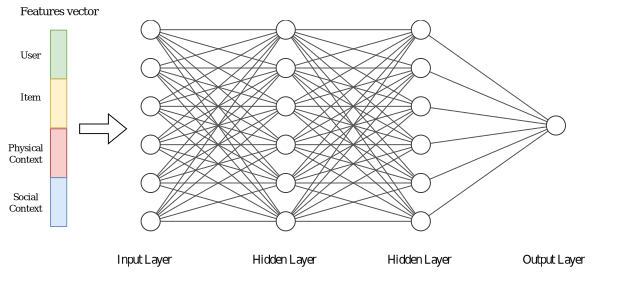
\includegraphics[width=\linewidth]{immagini/ffnet_schema.png}
  \caption{Schema rete feed-forward}
  \label{fig:ffnet_schema}
\end{figure}

% 
%			CAPITOLO 4: Datasets
% 

\chapter{Datasets}
\label{chap:datasets}


% 
%			CAPITOLO 5: Risultati
% 

\chapter{Risultati}
\label{chap:risultati}


% 
%			CAPITOLO 6: Conclusioni e sviluppi futuri
% 

\chapter{Conclusioni}
\label{cap6}

\section{Conclusioni}

Conclusioni...

\section{Sviluppi futuri}

Sviluppi futuri...



%
%			BIBLIOGRAFIA
%

\bibliographystyle{unsrt}
\bibliography{bibliografia}
\nocite{*}
\addcontentsline{toc}{chapter}{Bibliografia}


\end{document}


 
